\documentclass[a4paper,12pt,exos,firamath]{nsi}
		
\documentclass[a4paper,12pt,exos,firamath]{nsi}
		
\setminted{fontsize=\small}
\begin{document}
{\large\bfseries \scshape Nom Prénom : \makebox[6cm]{\dotfill}\hfill Heure de passage : \makebox[3cm]{\dotfill}\hfill\\
\vspace{2em}
\hrule
\vspace{2mm}
\begin{center}\titlefont\Huge\color{UGLiBlue} BTS SIO\\
	Sous-épreuve E22 \\ 
    Algorithmique appliquée\\
	Contrôle en Cours de Formation\end{center}
\vspace{2mm}
\hrule}
\vspace{2em}

\begin{encadrecolore}{Déroulement de l'épreuve }{UGLiGreen}
	Cette épreuve de Contrôle en cours de Formation (CCF) se déroule en trois étapes :
\begin{itemize}
	\item \textbf{\'Etape 1 : \'Ecrit (30 minutes)}\par
	Vous devez traiter la partie A du sujet. Pour cette partie, l'ordinateur est interdit mais la calculatrice est autorisée.\\
    
    \textbf{Vous inscrirez vos réponses dans le document réponse à la fin du sujet.}\\
    
    Les algorithmes à écrire peuvent être rédigés en \textbf{langage naturel} ou en \textsc{Python}	mais ni en \textsc{C\#} ni en \textsc{VB.Net}.\\
    
    \textbf{À la fin de l'étape 1, votre document réponse doit être remis à la personne surveillant l'épreuve.} Vous garderez le sujet.
    \item \textbf{\'Etape 2 : sur machine (30 minutes)}\par
	Vous devez traiter la partie B du sujet à l'aide d'un ordinateur. Le langage utilisé est celui travaillé dans l'année, à savoir \textsc{Python}.
	Vous sauvegarderez votre travail sur la clé USB fournie.\par 
	La durée totale pour effectuer les deux premières étapes est exactement d'une heure. \par
	\item \textbf{\'Etape 3 : oral (20 minutes au maximum)}\\
	Cette partie se déroule en deux temps. Tout d'abord, vous disposez de 10 minutes pour présenter votre travail de l'étape 2 puis, au cours des 10 minutes suivantes, un entretien permet de préciser votre démarche.
\end{itemize}	

\textbf{À la fin de l'épreuve le sujet devra être rendu à l'examinateur.}
\end{encadrecolore}
\newpage

\titre{Zoom}
\classe{CCF Algo SIO}
\maketitle

Une image rectangulaire en noir et blanc peut être représentée par une liste de lignes qui sont des listes d'entiers valant 0 (pour le noir) et 1 (pour le blanc).\\
Par exemple l'image suivante, de dimensions $5\times 4$
\begin{center}
    
\includegraphics[width=3cm]{img/fig1.png}
\end{center}

est représentée par la liste suivante :
\begin{minted}{python}
[[0, 0, 1, 0, 0], 
 [0, 1, 0, 1, 0],
 [0, 0, 1, 0, 0]]
\end{minted}

On aimerait construire une fonction \mintinline{python}{zoom} qui
\begin{itemize}
    \item en entrée prend une liste \mintinline{python}{lst} qui représente une image rectangulaire et un \mintinline{python}{int} strictement positif \mintinline{python}{k} ;
    \item renvoie une liste qui correspond à l'image représentée par \mintinline{python}{lst} grossie d'un facteur \mintinline{python}{k}.  
\end{itemize} 
Ci-dessous figure un exemple d'utilisation de la fonction \mintinline{python}{zoom}
\begin{center}
    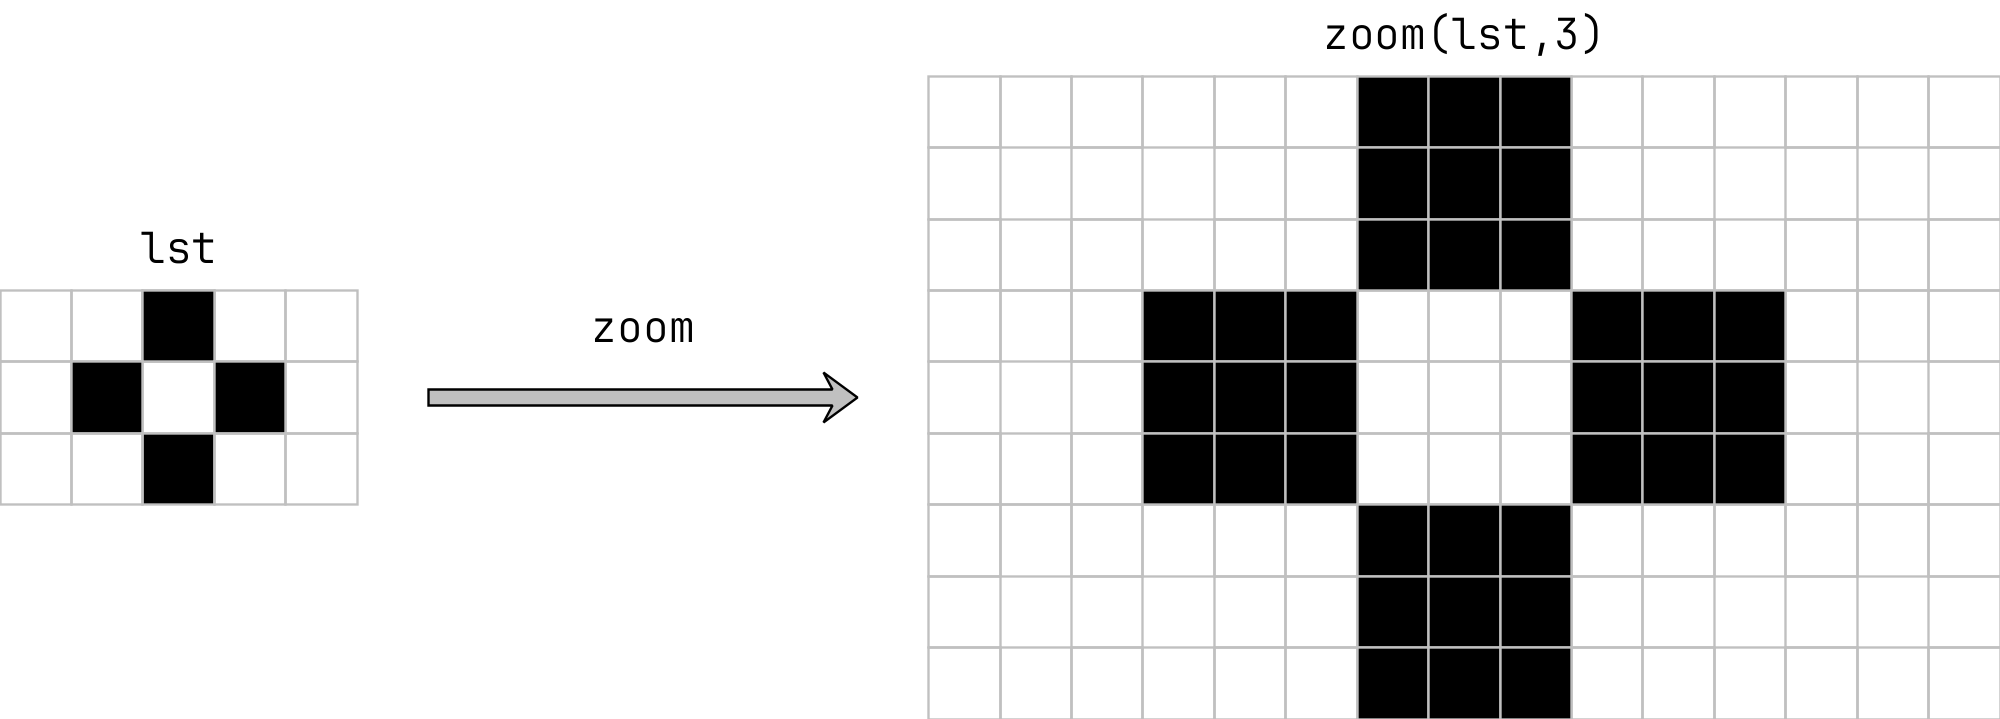
\includegraphics[width=14cm]{img/fig0.png}
\end{center}
\section*{Étape 1}

\begin{encadrecolore}{Question 1}{UGLiOrange}
	Dessiner l'image obtenue en appliquant \mintinline{python}{zoom(lst,2)} avec une liste \mintinline{python}{lst} représentant l'image suivante :
	\begin{center}
		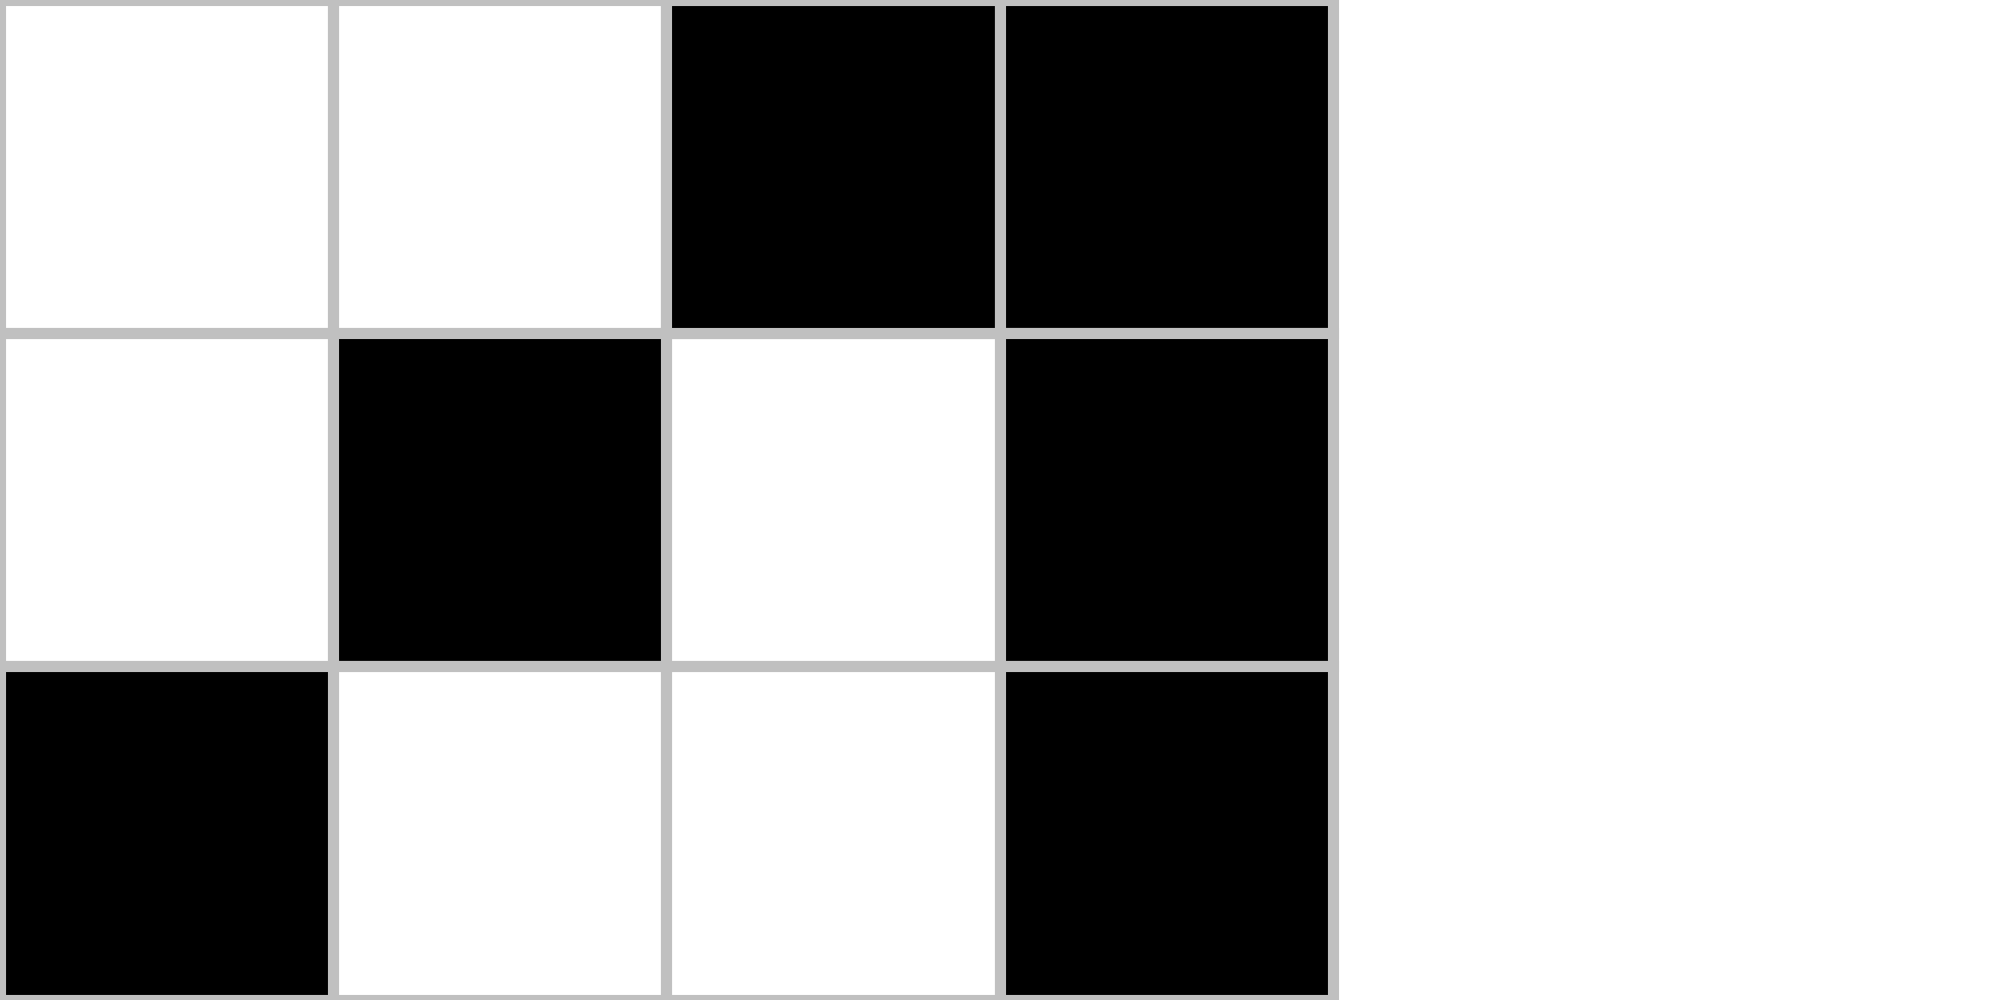
\includegraphics[width=2.8cm]{img/fig2.png}
	\end{center}	  
\end{encadrecolore}

\begin{encadrecolore}{Question 2}{UGLiOrange}
	Si \mintinline{python}{lst} représente une image de $n$ lignes par $p$ colonnes, et que \mintinline{python}{lst2 = zoom(lst, k)},  quelle est la taille de 
	\begin{enumerate}
		\item	\mintinline{python}{lst2} ? 
		\item	\mintinline{python}{lst2[0]} ? 
	\end{enumerate}
\end{encadrecolore}

\begin{encadrecolore}{Question 3}{UGLiOrange}
	Compléter le pseudocode de la fonction \mintinline{python}{zoom_horiz} qui


	\begin{minted}{pseudocode}
		fonction zoom(lst, k)
		
			variables
				résultat : liste
				valeur, compteur, i : entiers
				
			résultat ← liste vide
			n ← longueur(lst)
			pour i ...
			    pour j ...    
					ajouter ... à la fin de résultat
			renvoyer résultat
		\end{minted}
\end{encadrecolore}

\begin{encadrecolore}{Question 4}{UGLiOrange}
	Compléter le pseudocode de la fonction \mintinline{python}{zoom} que l'on veut coder
	\begin{itemize}
		\item	en entrée prend une liste d'entiers \mintinline{python}{ligne} et un entier \mintinline{python}{k} ; 
		\item	renvoie une liste d'entiers dans laquelle chaque valeur de \mintinline{python}{ligne} est dupliquée \mintinline{python}{k} fois.  
	\end{itemize} 

	\begin{minted}{pseudocode}
		fonction zoom_horiz(ligne, k)
		
			variables
				résultat : liste
				valeur, compteur, i : entiers
				
			résultat ← liste vide
			p ← longueur(ligne)
			pour i ...
			    pour j ...    
					ajouter ... à la fin de résultat
			renvoyer résultat
		\end{minted}
\end{encadrecolore}

\section*{Étape 2}
\begin{encadrecolore}{Question 5}{UGLiOrange}
	Ouvrir le fichier \mintinline{python}{zoom.py} et coder les fonctions manquantes.	
\end{encadrecolore}

\begin{encadrecolore}{Question 5}{UGLiOrange}
	Coder la fonction \mintinline{python}{affiche} qui
	\begin{itemize}
		\item en entrée prend une liste \mintinline{python}{lst} qui représente une image ;
		\item ne renvoie rien mais affiche joliment l'image avec des \mintinline{python}{'.'}  à la place des zéros et des \mintinline{python}{'*'} à la place des 1.
	\end{itemize} 
	On rappelle que \mintinline{python}{print('*', end="")} affiche \mintinline{python}{'*'} sans retour à la ligne.
\end{encadrecolore}


\end{document}